\documentclass[conference]{IEEEtran}
\IEEEoverridecommandlockouts
% The preceding line is only needed to identify funding in the first footnote. If that is unneeded, please comment it out.
\usepackage{cite}
\usepackage{amsmath,amssymb,amsfonts}
\usepackage{algorithmic}
\usepackage{graphicx}
\usepackage{textcomp}
\usepackage{xcolor}
\usepackage{floatrow}
\usepackage{caption}
\usepackage{wrapfig}
\usepackage{lipsum} % Pacote de exemplo para preencher o texto
\usepackage{url}

\def\BibTeX{{\rm B\kern-.05em{\sc i\kern-.025em b}\kern-.08em
    T\kern-.1667em\lower.7ex\hbox{E}\kern-.125emX}}
\begin{document}

\title{Predição de PIB em Países do Mundo
}

\author{
    \IEEEauthorblockN{
        João Vitor Bueno de Almeida \\
        Lucas Rocha Sahdo \\
        Renato Galli Barbosa Giglio
    }
    \IEEEauthorblockA{
        \textit{Universidade de Sorocaba} \\
        \textit{Graduação em Análise e Desenvolvimento de Sistemas e} \\ 
        \textit{Ciência de Dados e Inteligẽncia Artificial} \\   
        \textit{Disciplina Fundamentos de Ciência de Dados, Big Data e Inteligência Artificial} \\
        \textit{Prof. Me. Jaime Ranulfo Leite Filho} \\
        \textit{18023-000, Sorocaba, SP , Brasil}
    }
}

\maketitle

\renewcommand{\abstractname}{Resumo}

\begin{abstract}
Este estudo aborda a previsão do PIB per capita de países usando técnicas de aprendizado de máquina. O objetivo principal do estudo foi explorar os fatores que afetam o PIB per capita e desenvolver um modelo preditivo utilizando um conjunto de dados contendo informações socioeconômicas, demográficas e geográficas de 227 países. Inicialmente, realizamos análises exploratórias dos dados, identificamos valores ausentes e realizamos o pré-processamento necessário, como preenchimento desses valores faltantes e codificação das variáveis categóricas. Em seguida, dividimos o conjunto de dados em conjuntos de treinamento e teste e selecionamos as variáveis de treinamento e a variável alvo (GDP per capita). Utilizamos vários modelos de machine learning para realizar as predições, porém destacou-se o modelo de regressão por árvore de decisão. Avaliamos o desempenho do modelo utilizando métricas como R², MAE, MSE e RMSE, obtendo resultados promissores. Os resultados destacaram a importância de variáveis como população, densidade populacional, taxa de alfabetização e setores econômicos na previsão do PIB per capita. Este estudo contribui para a compreensão das relações entre variáveis socioeconômicas e o PIB per capita, além de demonstrar a aplicabilidade de técnicas de aprendizado de máquina nesse contexto. Espera-se que essas descobertas possam ser úteis para estudos futuros e para tomadores de decisão na área econômica.
\end{abstract}

\renewcommand{\IEEEkeywordsname}{Palavras-chave}

\begin{IEEEkeywords}
  PIB, economia, machine learning, random forest, Predição, Regressão Linear
\end{IEEEkeywords}

\section{Introdução}
A previsão do desempenho econômico é um desafio fundamental para a compreensão e tomada de decisões informadas em diferentes setores e países. A capacidade de prever o Produto Interno Bruto (PIB) de uma nação é de particular importância, pois fornece informações cruciais para políticas econômicas e investimentos estratégicos. Compreender as tendências e os fatores que influenciam o PIB per capita de um país pode auxiliar na alocação eficiente de recursos, planejamento de políticas de desenvolvimento e análise comparativa do desempenho econômico entre diferentes nações.

Neste contexto, a elaboração de um modelo preditivo de PIB per capita assume uma relevância significativa. Esse modelo possibilitaria a previsão do desempenho econômico futuro, considerando variáveis socioeconômicas, demográficas e geográficas. Ao obter projeções precisas do PIB per capita, tomadores de decisão podem direcionar investimentos, implementar políticas adequadas e promover o desenvolvimento sustentável. 

Além disso, a análise comparativa do desempenho econômico, utilizando as previsões geradas pelo modelo, permitiria uma compreensão mais profunda das diferenças significativas entre os países e as causas subjacentes a essas diferenças. Ao identificar padrões e tendências com base nos dados preditivos, seria possível examinar as políticas econômicas adotadas pelos países com melhor desempenho e extrair lições valiosas para aplicação em outras regiões. Esse conhecimento também poderia fortalecer a cooperação internacional e o intercâmbio de boas práticas, impulsionando o desenvolvimento econômico global.

O restante do artigo está estruturado da seguinte forma: na seção seguinte, apresentamos a metodologia utilizada, descrevendo o conjunto de dados, as etapas de pré-processamento, as técnicas de aprendizado de máquina empregadas e as métricas de avaliação do modelo. Em seguida, apresentamos os resultados obtidos e realizamos uma análise detalhada dos fatores relevantes para a previsão do PIB per capita. Por fim, discutimos as conclusões e as implicações práticas do estudo, destacando a importância dessas descobertas para a compreensão do desempenho econômico global e as possíveis aplicações futuras.

\section{Dados e Pré-Processamento}

\subsection{Dados}

Utilizou-se um conjunto de dados abrangente composto por informações socioeconômicas, demográficas e geográficas de 227 países ao redor do mundo. O objetivo principal da análise é desenvolver um modelo preditivo de PIB per capita, no qual essa variável representa nossa variável de interesse (Y).

O conjunto de dados é composto por diversas colunas que representam diferentes características dos países. Abaixo, apresentamos uma descrição resumida de cada uma dessas colunas:

\begin{itemize}
  \item \textbf{Country}: O nome do país.
  \item \textbf{Region}: A região geográfica à qual o país pertence.
  \item \textbf{Population}: A população total do país.
  \item \textbf{Area (sq. mi.)}: A área territorial do país em metros quadrados.
  \item \textbf{Pop. Density (per sq. mi.)}: A densidade populacional do país, ou seja, o número de habitantes por quilômetro quadrado.
  \item \textbf{Coastline (coast/area ratio)}: A relação entre a extensão da linha costeira e a área territorial do país.
  \item \textbf{Net migration}: A taxa líquida de migração, representando a diferença entre o número de imigrantes e emigrantes por 1.000 habitantes.
  \item \textbf{Infant mortality (per 1000 births)}: A taxa de mortalidade infantil, representando o número de mortes de crianças menores de um ano a cada 1.000 nascimentos.
  \item \textbf{GDP (\$ per capita)}: O PIB per capita do país, que é uma medida amplamente utilizada para avaliar o nível de desenvolvimento econômico.
  \item \textbf{Literacy (\%)}: A taxa de alfabetização da população adulta.
  \item \textbf{Phones (per 1000)}: O número de linhas telefônicas por 1.000 habitantes.
  \item \textbf{Arable (\%)}: A porcentagem de terras aráveis em relação à área territorial total.
  \item \textbf{Crops (\%)}: A porcentagem de terras cultivadas com culturas específicas em relação à área territorial total.
  \item \textbf{Other (\%)}: A porcentagem de terras não aráveis e não utilizadas em relação à área territorial total.
  \item \textbf{Climate}: Uma classificação numérica que indica o tipo de clima predominante no país.
  \item \textbf{Birthrate}: A taxa de natalidade, representando o número de nascimentos por 1.000 habitantes.
  \item \textbf{Deathrate}: A taxa de mortalidade, representando o número de mortes por 1.000 habitantes.
  \item \textbf{Agriculture}: A contribuição do setor agrícola para o produto interno bruto (PIB) do país.
  \item \textbf{Industry}: A contribuição do setor industrial para o PIB do país.
  \item \textbf{Service}: A contribuição do setor de serviços para o PIB do país.
\end{itemize}

Essas informações fornecem uma visão geral abrangente sobre os dados que foram utilizados nesta análise. Cada uma dessas variáveis apresenta um papel importante na determinação do PIB per capita dos países e será explorada em maior detalhe nas etapas subsequentes do estudo.

O mapa de calor da Figura 1 indica a correlação entre as variáveis X do estudo. Com base nas correlações calculadas entre o PIB per capita (GDP) e outras variáveis, podemos obter insights interessantes sobre a relação econômica e social dos países. Vamos analisar algumas dessas correlações específicas.

\begin{figure}[htbp]
  \centering
  \begin{floatrow}
    \ffigbox[\textwidth]{\caption{Mapa de Calor}\label{fig:imagem}}{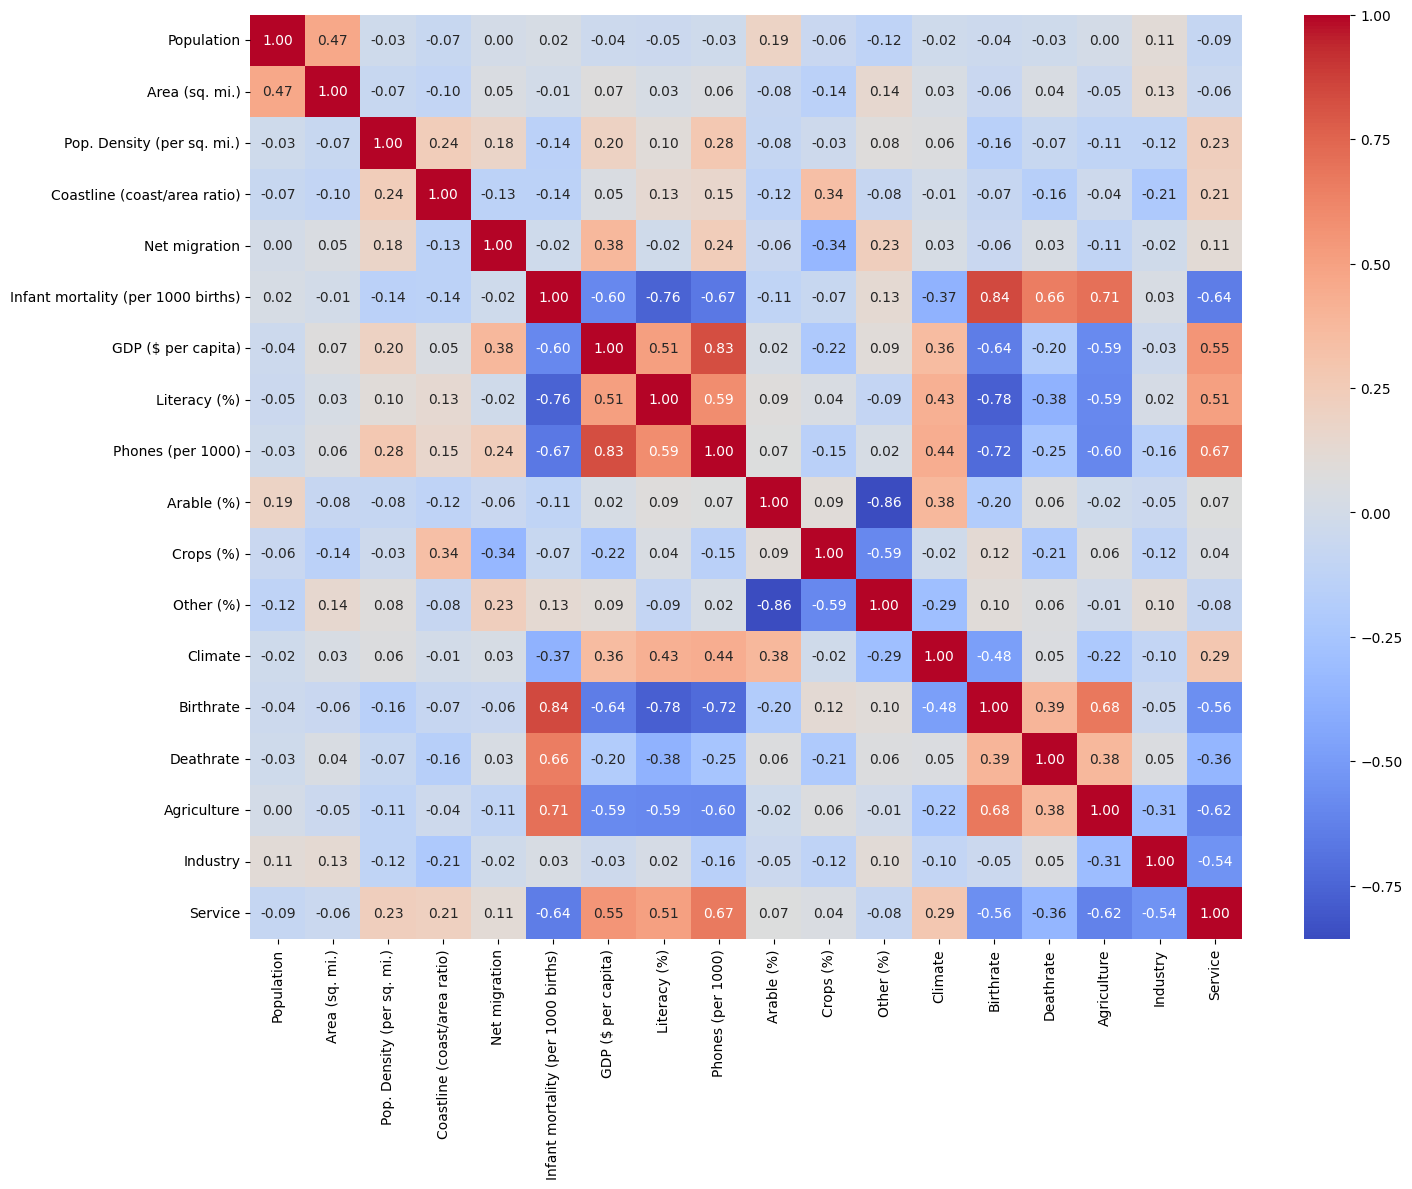
\includegraphics[width=1\textwidth]{img/calor.png}}
  \end{floatrow}
\end{figure}

A correlação positiva de 0.82 entre o PIB per capita e o número de linhas telefônicas por 1.000 habitantes (Phones) sugere uma associação significativa entre o desenvolvimento econômico e a infraestrutura de comunicação. Isso indica que países com maior acesso a serviços de telecomunicações tendem a ter um PIB per capita mais alto, possivelmente devido à influência positiva da tecnologia e das telecomunicações no crescimento econômico e no comércio.

A correlação de 0.51 entre o PIB per capita e a taxa de alfabetização da população adulta (Literacy) também é positiva, indicando que países com uma população mais alfabetizada tendem a apresentar um PIB per capita mais elevado. Isso sugere que a educação e o nível de alfabetização podem desempenhar um papel fundamental no desenvolvimento econômico, permitindo que as pessoas adquiram conhecimentos e habilidades necessários para impulsionar a produtividade e inovação em diferentes setores.

Por outro lado, observamos uma correlação negativa de -0.67 entre o PIB per capita e a taxa de mortalidade infantil (Infant mortality). Essa correlação sugere que países com uma taxa de mortalidade infantil mais baixa tendem a apresentar um PIB per capita mais alto. Isso pode ser atribuído a um melhor sistema de saúde e acesso a cuidados médicos de qualidade, o que contribui para a redução da mortalidade infantil e, por consequência, para um aumento no desenvolvimento econômico.

Outra correlação negativa significativa é de -0.64 entre o PIB per capita e a taxa de natalidade (Birthrate). Isso indica que países com uma taxa de natalidade mais baixa tendem a ter um PIB per capita mais elevado. Essa associação pode ser explicada pela existência de políticas eficientes de controle populacional, melhores condições socioeconômicas e maior acesso a serviços de saúde reprodutiva, que impactam positivamente o desenvolvimento econômico.

Além disso, podemos destacar as correlações negativas de -0.59 entre o PIB per capita e a contribuição do setor agrícola para o PIB (Agriculture), e a correlação positiva de 0.55 entre o PIB per capita e a contribuição do setor de serviços para o PIB (Service). Essas correlações indicam uma tendência de diversificação econômica, na qual países com uma economia mais voltada para os setores de serviços apresentam um PIB per capita mais elevado, enquanto aqueles com uma economia agrícola menos desenvolvida tendem a ter um PIB per capita mais baixo.

Essas correlações destacam a complexidade das interações entre fatores econômicos, sociais e demográficos, fornecendo insights valiosos sobre os determinantes do desenvolvimento econômico. No entanto, é importante ressaltar que correlações não implicam necessariamente em causalidade direta, e outros fatores podem influenciar essas relações. 

Uma outra forma de visualizar a relação entre as variáveis X e o PIB per capita (GDP) é por meio do gráfico de dispersão. Esse tipo de gráfico nos permite analisar a dispersão dos pontos no plano cartesiano, onde cada ponto representa a combinação dos valores de uma variável X e do PIB per capita.

\begin{figure}[htbp]
  \centering
  \begin{floatrow}
    \ffigbox[\textwidth]{\caption{Mapa de Dispersão}\label{fig:imagem}}{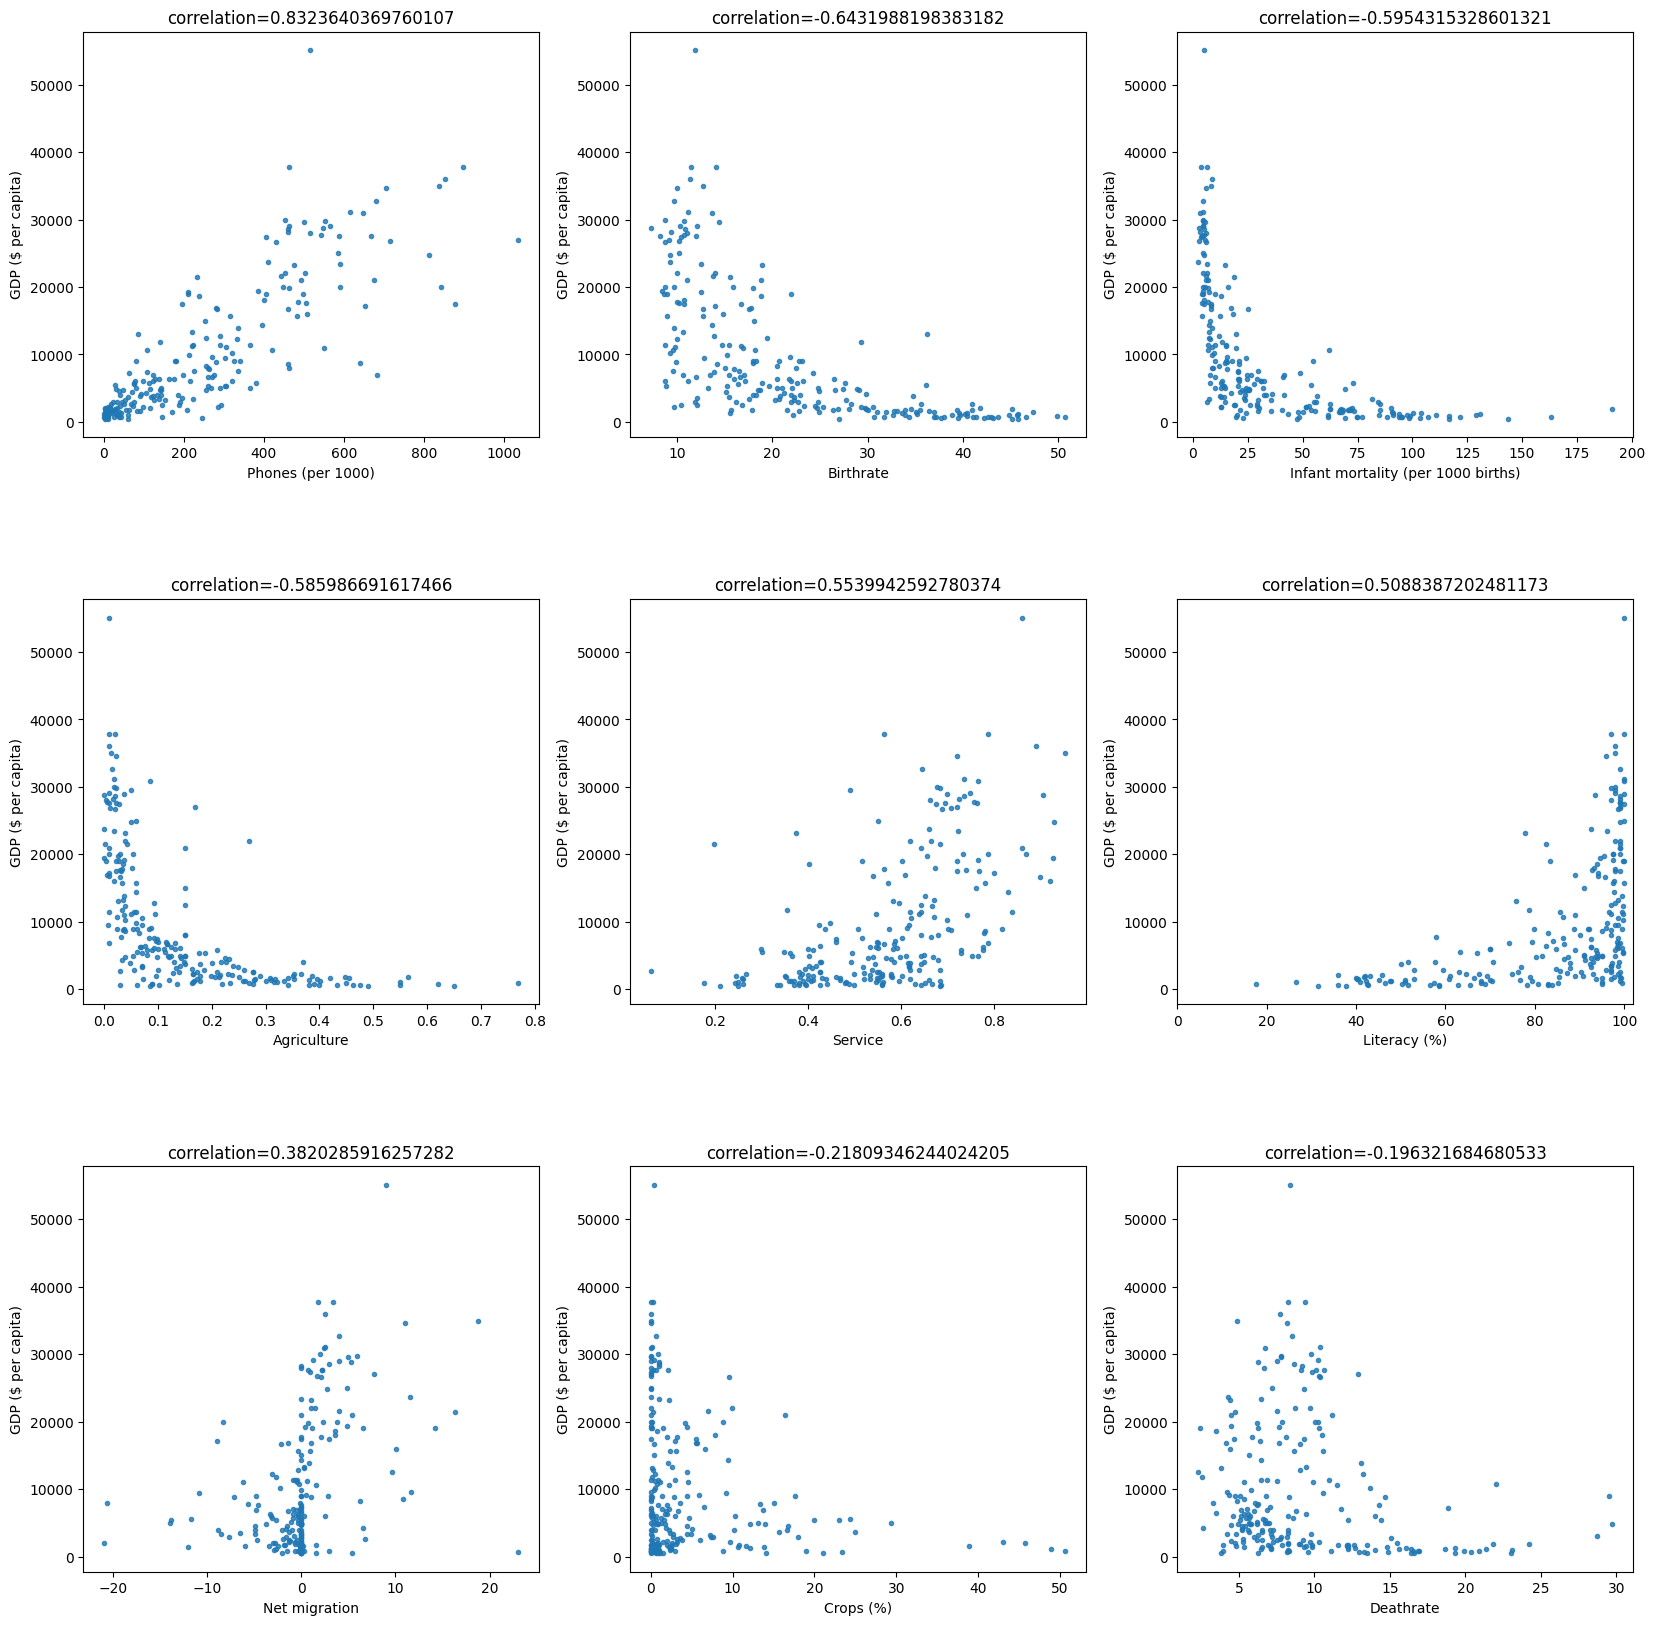
\includegraphics[width=1\textwidth]{img/dispersao.png}}
  \end{floatrow}
\end{figure}

No gráfico de boxplot apresentado na Figura 3, utilizamos a biblioteca Seaborn para visualizar a distribuição dos valores da coluna 'GDP (per capita)' do DataFrame 'df'. O eixo x representa a variável 'GDP (per capita)', que representa a renda per capita. O gráfico de boxplot é uma ferramenta estatística que nos permite observar a distribuição dos dados e identificar medidas resumidas importantes.

Esse gráfico nos permite visualizar a dispersão dos valores de renda per capita no conjunto de dados. É possível identificar a presença de valores extremos (outliers) e observar se a distribuição é simétrica ou assimétrica. Além disso, a mediana nos dá uma ideia do valor central da distribuição.

\begin{figure}[htbp]
  \centering
  \begin{floatrow}
    \ffigbox[\textwidth]{\caption{Renda Per Capta}\label{fig:imagem}}{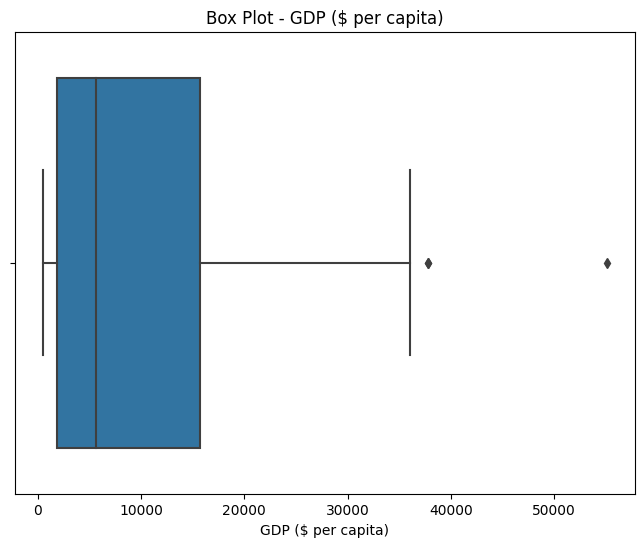
\includegraphics[width=1\textwidth]{img/renda_per_capta.png}}
  \end{floatrow}
\end{figure}

\subsection{Pré-processamento}

A fim de preparar os dados para análise, foram aplicados procedimentos de pré-processamento. Inicialmente, foi realizada a leitura de um arquivo CSV contendo os dados. Em seguida, foram verificados possíveis valores ausentes nos dados por meio da verificação de nulos em cada coluna do conjunto de dados.

Para tratar os valores faltantes, adotou-se uma abordagem baseada na mediana dos valores das colunas agrupadas por região. Ou seja, os valores ausentes foram preenchidos com a mediana correspondente à região em que o país se encontra. Esse método permite preservar a tendência central dos dados e minimizar o impacto de outliers ou valores extremos.

Após a imputação dos valores ausentes, uma etapa importante foi a análise da correlação entre as variáveis. Utilizando um mapa de calor, foi possível visualizar a matriz de correlação e identificar as relações entre as diferentes variáveis do conjunto de dados. Esse mapa de calor apresenta uma representação gráfica das correlações, sendo útil para identificar padrões e insights sobre as relações entre as variáveis.

Outra técnica de visualização utilizada foi o gráfico de boxplot, que permitiu analisar a distribuição dos valores da variável 'GDP (per capita)'. Essa representação gráfica mostrou a dispersão dos dados, incluindo informações sobre valores mínimos, quartis, mediana, quartis superiores e valores máximos, auxiliando na identificação de possíveis outliers ou valores discrepantes.

Adicionalmente, foram criados gráficos de barras e de dispersão para explorar a relação entre o PIB per capita e outras variáveis. O gráfico de barras destacou os 20 países com maior PIB per capita, oferecendo uma visualização clara das diferenças entre os países. Já o grid de gráficos de dispersão apresentou múltiplos gráficos de dispersão, cada um exibindo a correlação entre o PIB per capita e uma variável específica. Essa representação gráfica permitiu identificar relações lineares ou não lineares entre as variáveis e avaliar a força e direção dessas correlações.

\begin{figure}[htbp]
  \centering
  \begin{floatrow}
    \ffigbox[\textwidth]{\caption{Países com maior PIB per Capta}\label{fig:imagem}}{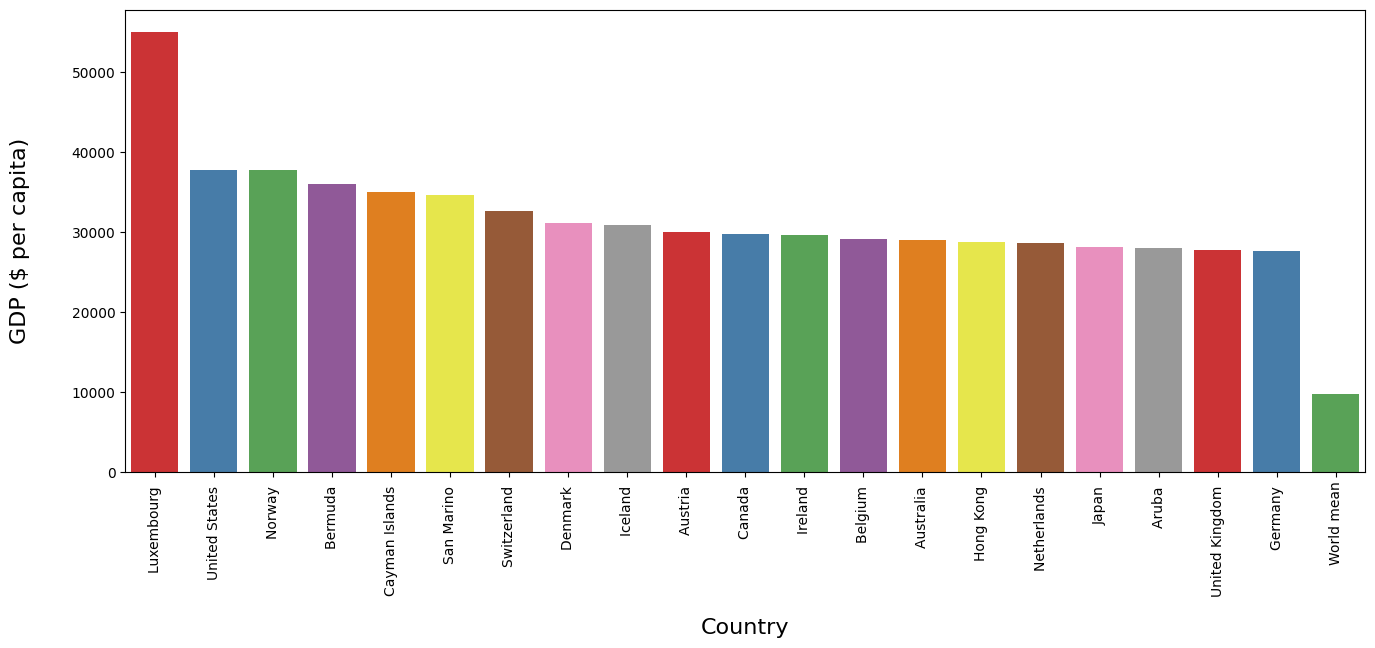
\includegraphics[width=1\textwidth]{img/20_rendas_paises.png}}
  \end{floatrow}
\end{figure}

Além das visualizações, algumas etapas adicionais de pré-processamento foram realizadas. Para possibilitar o uso de variáveis categóricas nos modelos de aprendizado de máquina, as variáveis 'Region' e 'Climate' foram codificadas utilizando a técnica LabelEncoder. Essa codificação transforma os valores categóricos em valores numéricos, permitindo a inclusão dessas variáveis nos modelos de regressão.

Por fim, o conjunto de dados foi dividido em conjuntos de treinamento e teste, e diversos algoritmos de machine learning foram avaliados para realizar o experimento. Dentre os algoritmos testados, o modelo baseado em Random Forest foi selecionado como o principal para este estudo. Utilizando as variáveis de treinamento e o PIB per capita como variável alvo, o modelo de Random Forest foi treinado e as previsões foram realizadas no conjunto de teste. Em seguida, foram analisadas métricas de desempenho, como R², MAE, MSE e RMSE, que fornecem informações sobre a qualidade das previsões realizadas pelo modelo de regressão e auxiliam na avaliação do seu desempenho.

\section{EXPERIMENTO E RESULTADOS}

Com o objetivo de garantir a reprodutibilidade dos resultados, neste trabalho são apresentadas as configurações adotadas para cada algoritmo de regressão linear, além de informações gerais sobre a base de dados e a metodologia experimental empregada.

Os experimentos foram projetados utilizando diferentes bibliotecas de aprendizado de máquina (ML) e análise de dados, incluindo o Scikit-Learn, Numpy e Pandas. Foram analisados seis algoritmos de ML: Regressão Linear (LinearRegression), Regressor de Árvore de Decisão (DecisionTree Regressor), Regressor de Floresta Aleatória (Random Forest Regressor) e Gradient Boosting.

Para a configuração experimental, devido à disponibilidade limitada de dados, não foi possível realizar uma etapa separada de validação. Assim, o conjunto de dados foi particionado em duas partes: uma para treinamento e outra para teste. A proporção utilizada foi de 70% para treinamento e 30% para teste.

Dessa forma, a abordagem adotada neste trabalho permite avaliar e comparar o desempenho dos diferentes algoritmos de ML considerados, utilizando uma metodologia consistente e padronizada. Apesar da ausência de uma etapa de validação separada, a avaliação do desempenho dos modelos no conjunto de teste ainda oferece insights valiosos sobre a capacidade de generalização dos algoritmos em relação aos dados não vistos previamente.

Essa estratégia auxilia na identificação do modelo mais adequado para a tarefa em questão, fornecendo informações importantes para a tomada de decisões e o aprimoramento de aplicações de aprendizado de máquina. É importante ressaltar que, em estudos futuros, a inclusão de uma etapa de validação pode fornecer uma avaliação ainda mais robusta e confiável dos modelos.

\begin{table}[htbp]
  \centering
  \caption{Resultados de R², MAE, MSE e RMSE para cada algoritmo utilizado.}
    \begin{tabular}{|l|r|r|r|r|}
    \hline
    \textbf{Algoritmo}           & \textbf{R²} & \textbf{MAE} & \textbf{MSE} & \textbf{RMSE} \\ \hline
    LR                           & 0.66        & 3444.84      & 31723419.76  & 5632.35       \\ \hline
    DR                           & 0.65        & 3504.34      & 33178550.72  & 5760.08       \\ \hline
    RF                           & 0.89        & 2128.14      & 10236560.49  & 3199.46       \\ \hline
    GB                           & 0.84        & 2436.99      & 14821628.31  & 3849.88       \\ \hline
    \end{tabular}%
  \label{tab:resultados}%
\end{table}%

Com base nos resultados obtidos e apresentados na Tabela \ref{tab:resultados}, concluímos que o algoritmo Random Forest (RF) se destacou como a melhor opção para o problema de regressão analisado neste estudo. O RF obteve um valor de R² de 0.89, o que indica que aproximadamente 89\% da variabilidade da variável dependente foi explicada pelas variáveis independentes consideradas no modelo.

Além disso, o RF demonstrou um desempenho superior em relação aos outros algoritmos testados, apresentando os menores valores de MAE, MSE e RMSE. Isso significa que as previsões geradas pelo modelo RF apresentaram uma menor discrepância em relação aos valores reais, resultando em um melhor ajuste aos dados observados.

Portanto, com base nessas métricas de desempenho, podemos afirmar que o algoritmo Random Forest é uma escolha promissora para tarefas de regressão, oferecendo uma boa capacidade de previsão e explicação da variabilidade dos dados.

No entanto, é importante ressaltar que a escolha do algoritmo mais adequado depende das características específicas do problema em questão, e diferentes algoritmos podem apresentar melhores resultados em diferentes cenários. Portanto, é sempre recomendado realizar uma análise cuidadosa e considerar outros fatores relevantes ao selecionar o algoritmo mais apropriado para uma determinada tarefa de regressão.

\begin{table}[h]
\centering
\caption{Resultados do Cross Validation}
\begin{tabular}{|c|c|}
\hline
Fold & Score \\
\hline
1 & 0.8796445693574401 \\
2 & 0.707313268755632 \\
3 & 0.7720971988186387 \\
4 & 0.6963693287169093 \\
5 & 0.7094417946315039 \\
\hline
\end{tabular}
\end{table}


\begin{figure}[htbp]
  \centering
  \begin{floatrow}
    \ffigbox[\textwidth]{\caption{Média dos Scores}\label{fig:imagem}}{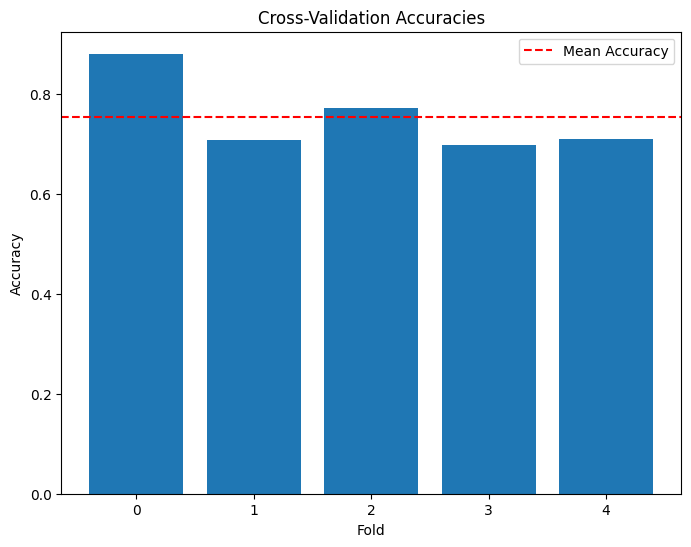
\includegraphics[width=1\textwidth]{img/media_dos_scores.png}}
  \end{floatrow}
\end{figure}

Ao avaliar a precisão das previsões do modelo, foram calculadas outras métricas importantes. O erro absoluto médio (MAE) foi encontrado como 2128.14, representando a média das diferenças absolutas entre as previsões e os valores reais. O erro quadrático médio (MSE) foi calculado em 10236560.49, sendo uma média dos erros ao quadrado. A raiz quadrada do erro quadrático médio (RMSE) foi determinada como 3199.46, representando o desvio padrão dos erros entre as previsões e os valores reais.

Esses resultados sugerem que o modelo de regressão Random Forest aplicado neste trabalho apresentou um desempenho consideravelmente bom na tarefa de previsão. Os valores de R², MAE, MSE e RMSE indicam a capacidade do modelo de explicar a variabilidade dos dados de teste e a magnitude dos erros nas previsões, respectivamente. Essas métricas são essenciais para avaliar e comparar o desempenho de diferentes modelos e podem auxiliar na seleção do modelo mais adequado para aplicações futuras.

\section*{Conclusão}

Com base nos resultados apresentados na tabela, podemos concluir que o algoritmo Random Forest (RF) obteve o melhor desempenho em termos de R², MAE, MSE e RMSE. O RF alcançou um valor de R² de 0.89, indicando que aproximadamente 89% da variabilidade da variável dependente foi explicada pelas variáveis independentes consideradas no modelo.

Além disso, o RF apresentou os menores valores de MAE, MSE e RMSE em comparação com os demais algoritmos testados. Isso significa que as previsões geradas pelo RF tiveram menor erro médio, menor dispersão dos erros e menor raiz quadrada do erro médio em relação aos valores reais.

Esses resultados indicam que o algoritmo Random Forest é altamente eficaz na tarefa de regressão para o conjunto de dados em análise. Sua capacidade de capturar padrões complexos e realizar uma combinação de múltiplas árvores de decisão resultou em um desempenho superior na explicação e previsão dos dados.

Portanto, com base nesses resultados, podemos afirmar que o algoritmo Random Forest é a escolha mais adequada para esse conjunto de dados, oferecendo um bom equilíbrio entre precisão e capacidade de generalização. No entanto, é importante ressaltar que a escolha do algoritmo deve considerar as características específicas do problema e a natureza dos dados.

\renewcommand{\refname}{Referências}

\begin{thebibliography}{00}
\bibitem{b1} Rodella, V.G. (2023). "Estudo de caso: Aplicação de Machine Learning para a previsão de tendências das ações das bolsas de valores brasileira e norte americana." Disponível em: \url{https://repositorio.unesp.br/bitstream/handle/11449/239653/rodella_vg_tcc_soro.pdf?sequence=7}
\bibitem{b2} DS Academy. (2023). "10 Casos de Uso de Machine Learning em Finanças." Disponível em: \url{https://blog.dsacademy.com.br/10-casos-de-uso-de-machine-learning-em_financas/}
\bibitem{b3} Google Colaboratory. Disponível em: \url{https://colab.research.google.com/}
\bibitem{b4} Kaggle. Disponível em: \url{https://www.kaggle.com/}
\bibitem{b5} Python. Disponível em: \url{https://www.python.org/}
\bibitem{b6} Udemy. (2023). "Machine Learning and Data Science with Python and Kaggle | A-Z." Disponível em: \url{https://www.udemy.com/course/machine-learning-data-science-with-python-kaggle-a-z/}
\bibitem{b7} InsightLab UFC. (2022). "Principais algoritmos de Machine Learning para você conhecer em 2022." Disponível em: \url{https://www.insightlab.ufc.br/principais-algoritmos-de-machine-learning-para-voce-conhecer-em-2022/}
\bibitem{b8} DataGeeks. (2019). "Principais algoritmos de machine learning." Disponível em: \url{https://www.datageeks.com.br/algoritmos-de-machine-learning/}
\end{thebibliography}
\vspace{12pt}
\end{document}